
%\title{LaTeX Portrait Poster Template}
%%%%%%%%%%%%%%%%%%%%%%%%%%%%%%%%%%%%%%%%%
% a0poster Portrait Poster
% LaTeX Template
% Version 1.0 (22/06/13)
%
% The a0poster class was created by:
% Gerlinde Kettl and Matthias Weiser (tex@kettl.de)
% 
% This template has been downloaded from:
% http://www.LaTeXTemplates.com
%
% License:
% CC BY-NC-SA 3.0 (http://creativecommons.org/licenses/by-nc-sa/3.0/)
%
%%%%%%%%%%%%%%%%%%%%%%%%%%%%%%%%%%%%%%%%%

%----------------------------------------------------------------------------------------
%   PACKAGES AND OTHER DOCUMENT CONFIGURATIONS
%----------------------------------------------------------------------------------------

\documentclass[a0,portrait]{a0poster}

\usepackage{multicol} % This is so we can have multiple columns of text side-by-side
\columnsep=100pt % This is the amount of white space between the columns in the poster
%\columnseprule=3pt % This is the thickness of the black line between the columns in the poster

\usepackage{xcolor}
\usepackage{url}
\usepackage{times} % Use the times font
%\usepackage{palatino} % Uncomment to use the Palatino font

\usepackage{graphicx} % Required for including images
\graphicspath{{figures/}} % Location of the graphics files
\usepackage{booktabs} % Top and bottom rules for table
\usepackage[font=normalsize,labelfont=bf]{caption} % Required for specifying captions to tables and figures
\usepackage{amsfonts, amsmath, amsthm, amssymb} % For math fonts, symbols and environments
\usepackage[top=2in, bottom=1.5in, left=2in, right=2in]{geometry}
\usepackage{wrapfig} % Allows wrapping text around tables and figures
\usepackage[none]{hyphenat} 

\usepackage{hyperref}
\usepackage{url}
\usepackage{breakurl}

%%%%%%%%%%%%%%%%%%%%%%%%%%%%%%%%%%%%%%%%%%%%%%%%%%%%%%%%%%%
%Section environment definition (boxes)

\definecolor{fillcol}{RGB}{255,255,255}			%Fill-colour of box
\definecolor{boxcol}{RGB}{222,31,38}
\fboxsep=1cm							%Padding between box and text
\fboxrule=2mm							%Width of box outline
\renewcommand{\rmdefault}{ppl}			%Reset serif to Palatino
\setlength{\columnsep}{2cm}		
\newsavebox\envbox 					%Define name for boxes used
\newenvironment{Section}[1]{
\par 
\flushleft
\colorbox{boxcol}{ 				%Draws solid colour box around title
\sffamily\large\color{black} #1%Typesets section name
\hspace{0.5cm}}
\par\nobreak 
\nointerlineskip 						%Fits title snugly above box (no gap)
\setlength\parskip{-1pt}					%Even snugger
\begin{lrbox}\envbox						%Opens box environment
\begin{minipage}{0.95\columnwidth}		%Opens minipage environment for section contents
}
{\par
\end{minipage}\end{lrbox}				%Close minipage and box
\fcolorbox{boxcol}{fillcol}{\usebox\envbox}	%Draw box with contents frame colour: boxcol, fill colour: fillcol
\vspace{1cm}							%Add spacing below box
} 
%%%%%%%%%%%%%%%%%%%%%%%%%%%%%%%%%%%%%%%%%%%%%%%%%%%%%%%%%%%



\begin{document}

%\fontsize{35}{35}\selectfont 
\fontsize{28}{30}\selectfont 

%----------------------------------------------------------------------------------------
%   POSTER HEADER 
%----------------------------------------------------------------------------------------

% The header is divided into two boxes:
% The first is 75% wide and houses the title, subtitle, names, university/organization and contact information
% The second is 25% wide and houses a logo for your university/organization or a photo of you
% The widths of these boxes can be easily edited to accommodate your content as you see fit

\begin{minipage}[t]{0.75\linewidth}
%\VERYHuge \color{boxcol} \textbf{Towards understanding the role of repeat elements in genome biology} \color{black}\\[0.5cm] % Title
\veryHuge \color{boxcol} \textbf{Wanderer} \color{black}\\[-2cm] % Title

%\veryHuge\textit{A semantic approach}\\[2cm] % Subtitle
\Huge\textit{An interactive viewer to explore DNA methylation and gene expression data in human cancer}\\[-1cm] % Subtitle

\LARGE \textbf{Anna D{\'i}ez-Villanueva, Izaskun Mallona \& Miguel A. Peinado}\\[0.5cm] % Author(s)
\LARGE Institute of Predictive and Personalized Medicine of Cancer (IMPPC) \\[0.4cm] % University/organization
\LARGE Health Science Research Institute of the Germans Trias i Pujol Foundation (IGTP) \\[0.4cm] % University/organization

\end{minipage}
%
\begin{minipage}[t][4em][c]{0.25\linewidth}
\textcolor{white}{qqqqqqqqqqqq qqqqqqqqqqqq qqqqqqqqqqqq qqqqqqqqqqqq qqqqqqqqqqqq qqqqqqqqqqqq qqqqqqqqqqqq qqqqqqqqqqqq qqqqqqq qqqqqqqqqqqqqqqq qqqqqqqqqqqq qqqqqqqqqqqq qqqqqqqqqqqq qqqqqqqqqqqq qqqqqqqqqqqq qqqqqqqqqqqq qqqqqqq qqqqqqqqqqqqqqqq qqqqqqqqqqqq qqqqqqqqqqqq qqqqqqqqqqqq qqqqqqqqqqqq qqqqqqqqqqqq qqqqqqqqqqqq qqqqqqq qqqq}
\includegraphics[width=20cm]{figures/logo_imppc_igtp.png}\\
\end{minipage}



\vspace{1cm} % A bit of extra whitespace between the header and poster content

%----------------------------------------------------------------------------------------


\begin{multicols}{2} % This is how many columns your poster will be broken into, a portrait poster is generally split into 2 columns

%\begin{Section}{\textbf{The importance of DNA methylation}}

%Cytosine methylation in CpG dinucleotides is an important mechanism involved in the regulation of multiple biological processes. Bisulfite-treated DNA sequencing is the gold standard technique to determine DNA methylation at the single CpG level. The functional implications of DNA methylation states are often determined at the regional level, therefore, the interpretation require further analysis that is highly benefited by the implementation of visualization tools.\\

%\end{Section}




%----------------------------------------------------------------------------------------

\vspace{-14cm}

\begin{Section}{\textbf{The Cancer Genome Atlas enormous data availability}}
% Data analysis on human cancer is a hotspot in basic and clinical research. As a group of largely heterogenous and complex disease, cancer research is benefited by coordinated efforts on data acquisition and analysis. The Cancer Genome Atlas (TCGA) is a result of an international effort that offers a multilayered view of the genomics and epigenomics of more than 30 human cancer types. This enormous data availability opens a wide world of possibilities to the research community. For instance, it allows \textit{in silico} hypothesis testing or validation of in-house results through an independent series.\\

The Cancer Genome Atlas (TCGA) initiative is an ambitious project aiming to accelerate our understanding of the molecular basis of cancer by providing large-scale genome information from thousands of clinically characterized cancer samples. The complex and comprehensive  nature of the generated data represents a privileged opportunity for researchers to get insights into the molecular landscapes of cancers. In fact, the landmark papers reporting the original data of each tumor type may just be considered a modest anticipation of the expected overall outcome.\\

Nevertheless,  wet lab experimentalists have very limited access to these data because sophisticated bioinformatic skills are required to manage and analyze such large datasets. Hence, development of interfaces facilitating the visualization and analysis of the information to non-bioinformaticians is essential to get a broad exploitation of this gigantic effort.\\


As experimental researchers with a long track of investigations using both candidate oriented and exploratory type studies, we are fully aware of these shortcomings. Our response has been the development of Wanderer, a very simple and intuitive web tool allowing real time access and visualization of \textbf{gene expression and DNA methylation profiles from TCGA data using gene targeted queries}.\\


\end{Section}


%----------------------------------------------------------------------------------------


% \begin{Section}{\textbf{Need of an user-friendly gateway to the data}}


% \end{Section}

\begin{Section}{\textbf{Wanderer, a ready-to-go TCGA data viewer}}

% With this aim we developed a tool, the TCGA Wanderer, that allows to easily retrieve and visualize the regional profiles of groups of samples belonging to a tumor type. The user is only asked to introduce the TCGA dataset (i.e. colon adenocarcinoma), whether the query is related to methylation (Illumina 450k) or expression (RNAseq), and gene symbol or Ensembl ID are valid target identifiers. The result layout summarizes in a upper panel the normal's profile and the lower, the tumor's. Each profile links by lines the selected values by sample, meaning that sample heterogeneity may be easily inspected by eye. Gene location and sense and CpG islands (for methylation plots) are also printed. The plots are highly dynamic, allowing to move through a region and to zoom in and out. Images and the TCGA's data they represent are downloadable just by clicking a button. Currently the we have 19 different datasets available: colon adenocarcinoma (COAD), breast invasive carcinoma (BRCA), lung adenocarcinoma (LUAD) and thyroid carcinoma (THCA), among others.  \\


For any given gene selected by the investigator, the tool provides detailed individual profiles of gene expression, exon by exon, and DNA methylation of all the probes inside or in the vicinity of the gene. Graphs for normal and tumor samples from any of the 19 available TCGA datasets are readily produced. Summarizing plots and tables are also generated, allowing further data analysis or representation using any software the investigator is used to (e.g.: Excel or any other spreadsheet or graphing tool). In addition, statistical analysis is applied to identify differential gene expression or DNA methylation between normal and tumor samples at either the single exon or the DNA methylation probe level, respectively. The tool allows local navigation and zoom in/out within the region of interest, as well as simple graph customization. Resulting graphs and tables may be downloaded and an application programming interface (API) allows data sharing, automatable query of multiple instances and direct linkage from external servers.\\


\end{Section}



% \begin{Section}{\textbf{Usage examples}}


% Some example of issues that can be resolved by querying Wanderer (and not easily reachable without this tool) include:
% \begin{itemize}
% \item Are different samples expressing the same gene isoforms? Which exon(s) should I analyze to find the largest difference between normal and tumor? See example in Figure \ref{fig:2}.
% \item Which region of the CpG island should I analyze to find the largest abnormal DNA methylation in tumor samples? Is it the same for different tumor types? See example in Figure \ref{fig:3}.
% \item Are methylation changes in the CpG island of my favorite gene specific? Or rather, are they consequence of a regional phenomenon? See example in Figure \ref{fig:4}.
% \end{itemize}

% \end{Section}





\begin{Section}{\textbf{Use case: Exon differential expression visualization}}

  \begin{center}\vspace{1cm}
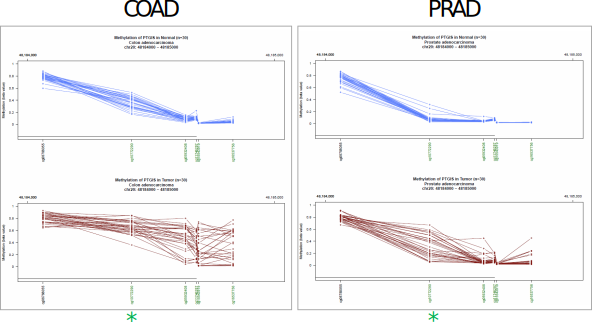
\includegraphics[width=\linewidth]{./figures/fig3.pdf}
\captionof{figure}{
DNA methylation profile of PTGIS CpG island in Colon adenocarcinomas (COAD) and Prostate adenocarcinomas (PRAD). Note that cg1077290 probe (*) is already very methylated in colon normal tissue, offering poor discriminat resolution to detect tumor hypermethylation compared with the rest of CpG island probes (labeled in green). In contrast, this probe (cg1077290) shows the highest level of hypermethylation in Prostate cancers (PRAD) and remains unmethylated in normal, resulting as the most discriminant variable in tis type of cancer.
}
\end{center}\vspace{1cm}

  
\end{Section}



\begin{Section}{\textbf{Easy-to-use user interface}}

  \begin{center}\vspace{1cm}
\includegraphics[width=\linewidth]{./figures/fig1.pdf}
\captionof{figure}{
Snapshot of Wanderer webpage. Boxes indicate the different panels for gene name/ID and dataset selection (a), view customization (b and c), output (d) and data download and links (e).
}
\end{center}\vspace{1cm}

  
\end{Section}


% \begin{Section}{\textbf{Graphical user interface}}

%   \begin{center}\vspace{1cm}
% 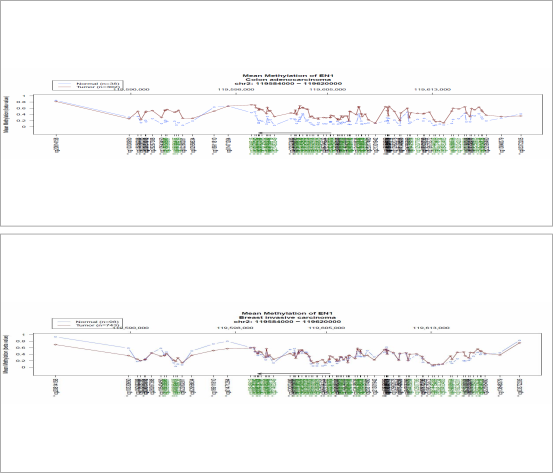
\includegraphics[width=\linewidth]{./figures/fig4.pdf}
% \captionof{figure}{
% DNA methylation profile of the genomic region flanking the EN1 gene. Note the large number of CpG islands (green probes) and that in Colon  adenocarcinomas (COAD),the whole region is hypermethylated, while in Breast cancer,  regions of hypomethylation and hypermethylation may be observed. The graphs display the average methylation values of each dataset. Probes marked with an asterisk denote statistically significant differences between normal and tumor samples.

% }
% \end{center}\vspace{1cm}

  
% \end{Section}



% \begin{figure}[center]
%   \centering
%   \includegraphics[width = \textwidth]{fig1.pdf}
%   \caption{Snapshot of Wanderer webpage. Boxes indicate the different panels for gene name/ID and dataset selection (a), view customization (b and c), output (d) and data download and links (e). Web access to Wanderer: \href{http://www.maplab.cat/betawanderer}{http://www.maplab.cat/betawanderer}.}
%   \label{fig:1}
% \end{figure}



\begin{Section}{\textbf{Availability}}

The user-friendly web application has been developed using R/shiny and is freely accesable at \url{maplab.cat/betawanderer} (provisional address). As it is hosted in a shiny server, the final user only needs a web browser to run it and requires no installation, being platform-indepedent and runnable on commodity computers, such as low-memory laptops.\\

  
\end{Section}





% \begin{Section}{\textbf{Even more random text}}

% \begin{center}\vspace{1cm}
% % \includegraphics[width=0.8\linewidth]{./figures/protege_clouds.pdf}
% % \captionof{figure}{
% % As reflected by tag cloud views, the most abundant class properties (top left) show how different classes (top right) are linked. For instance, \texttt{closest chromatin state to Alu} is a highly used property as well \texttt{8 Insulator} is a common chromatin state. However, some data is attached to given classes as simple attributes (bottom left), such as the genomic location. Finally, all the terms have an explicit hierarchy (bottom right). 
% % }
% \end{center}\vspace{1cm}


% \end{Section}


%\begin{Section}{\textbf{Acknowledgements}}
\begin{small}
This work was supported by grants from the Spanish Ministry of Economy and Knowledge (SAF2011/23638, PTA2011-5655-I) and from Generalitat de Catalunya (2009 SGR1356).\\
\end{small}
%\end{Section}


\end{multicols}
\end{document}            


